\documentclass [handout] {beamer}
\usepackage[T1]{fontenc}
\usepackage[english]{babel}
\usepackage{hyperref}
\usepackage{graphicx}
\usepackage{caption}
\usepackage{amsmath}
\captionsetup{figureposition=bottom, font=small}
\usetheme{Warsaw}
\usecolortheme{crane}
\newtheorem{formula}{}{}

\title{Deblurring Images with Neural Networks}
\author{Francesco Bonzi and Andrea Zanellati}
\institute{Deep Learning Course Project \\
	\medskip
	\textit{prof. Andrea Asperti}
}
\date{\today\  \\ }

\begin{document}

\begin{frame}
	\titlepage
\end{frame}

\begin{frame}
	\frametitle{Autoencoder}
	\begin{formula}
		An autoencoder is an artificial neural network that learns to copy its input to its output
	\end{formula}
	\begin{columns}
		\begin{column}{0.4\textwidth}
			\begin{figure}[]
			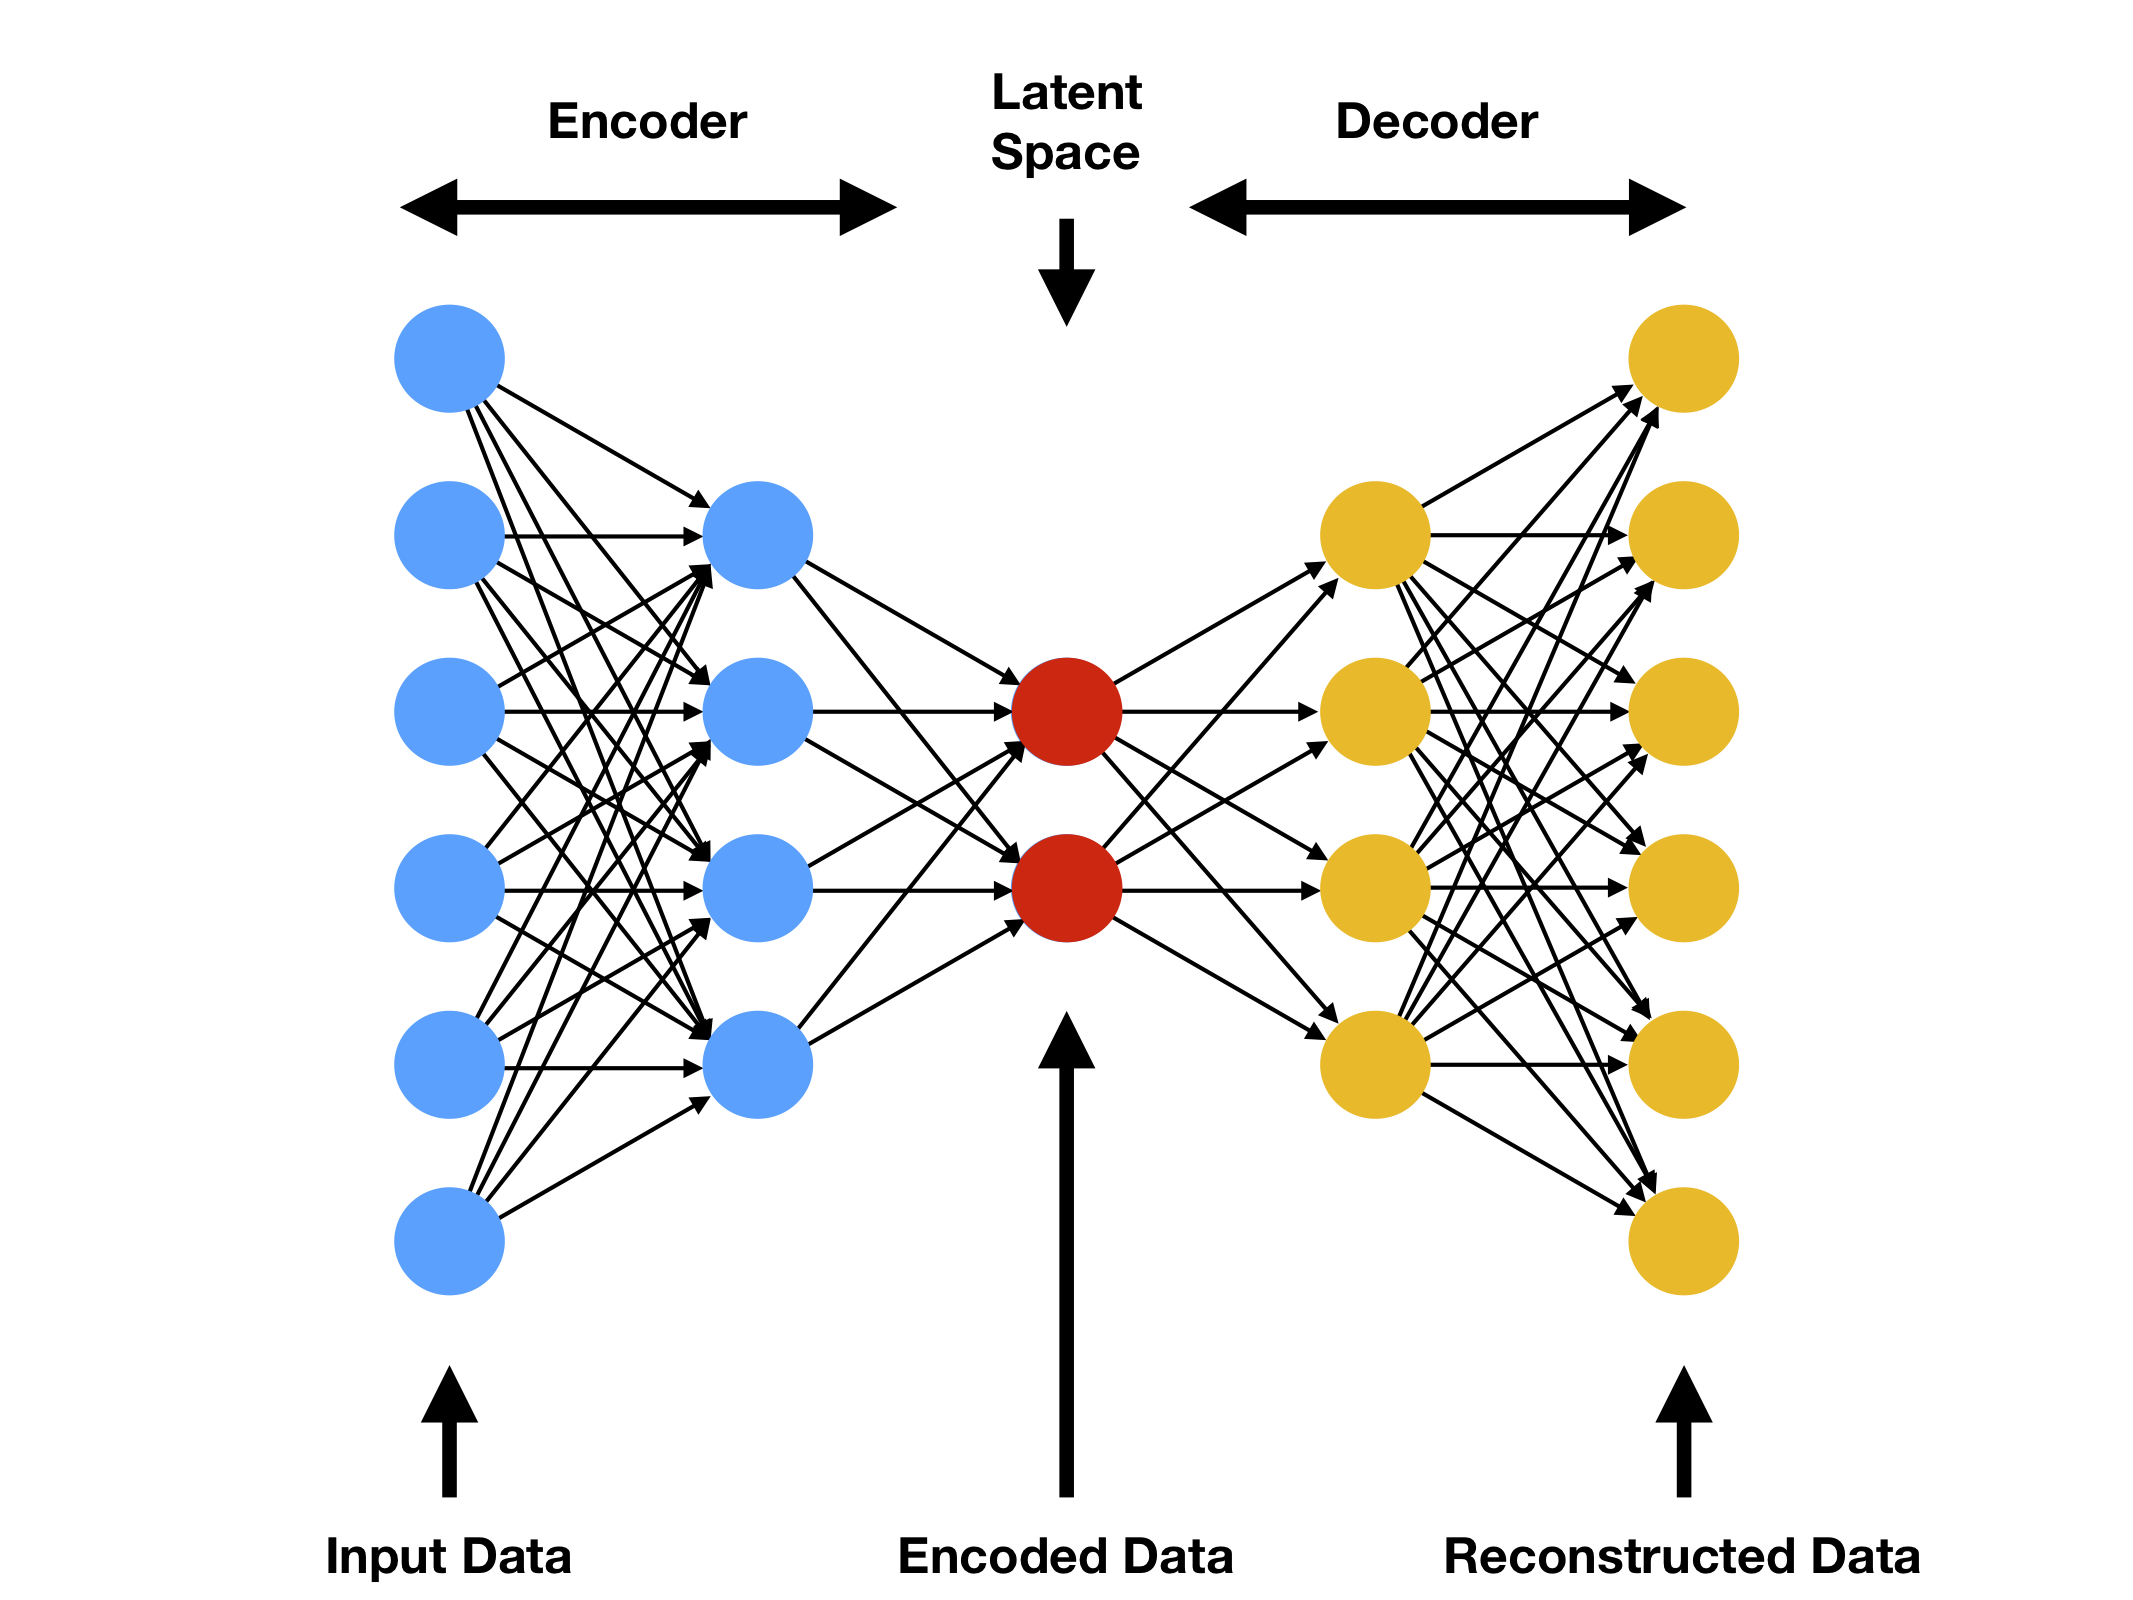
\includegraphics[width=1.3\columnwidth]{autoencoder_model.png}
    			\caption{autoencoder model}
			\end{figure}
		\end{column}
		\begin{column}{0.4\textwidth}
			Models:
			\begin{itemize}
				\item \textit{Plain Network}
				\item \textit{Skip Connections}
				\item \textit{ResNet}
			\end{itemize}
		\end{column}
	\end{columns}
\end{frame}

\begin{frame}
	\frametitle{Plain Network}
	3 models:
	\begin{equation}
		C_{32}^{3,1} - C_{64}^{3,1} - C_{128}^{3,1} - D_{128}^{3,1} - D_{64}^{3,1} - D_{32}^{3,1} - D_{3,p}^{3,1} 
		\label{CNNbase_v1}
	\end{equation}
	\medskip
	\begin{equation}
		5C_{8}^{3,1} - 5C_{16}^{3,1} - 5C_{32}^{3,1} - 5D_{32}^{3,1} - 5D_{16}^{3,1} - 5D_{8}^{3,1} - D_{3,p}^{3,1} 
		\label{CNNbase_v2}
	\end{equation}
	\medskip
	\begin{equation}
		4C_{16}^{3,1} - 4C_{32}^{3,1} - 4C_{64}^{3,1} - 4D_{64}^{3,1} - 4D_{32}^{3,1} - 4D_{16}^{3,1} - D_{3,p}^{3,1} 
		\label{CNNbase_v2}
	\end{equation}
	\begin{figure}[hbtp]
		\centering
		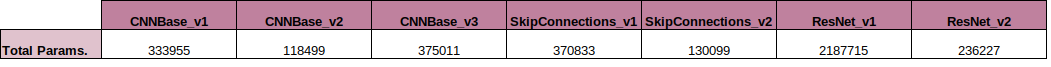
\includegraphics[scale=0.35]{params_table.png}
		\caption{Table of the toltal number of parameters in each network}\label{table_params}
	\end{figure}
\end{frame}

\begin{frame}
	\frametitle{Skip Connections}
	2 models:
	\begin{equation}
	\begin{split}
		C1_{32}^{3,1} - C2_{64}^{3,1} - C3_{64}^{3,1} - C4_{128}^{3,1} - \\ D5_{128}^{3,1} - D6_{64}^{3,1} - S7_{C2} - D8_{32}^{3,1} - S9_X - D10_{3,p}^{3,1} 
	\end{split}
	\end{equation}
	\medskip
	\begin{equation}
	\begin{split}
		5C_{8}^{3,1} - 10C_{16}^{3,1} - 5C_{32}^{3,1} - 5D_{32}^{3,1} - 5D_{16}^{3,1} - S_{C6} - \\ 2D_{8}^{3,1} - S_{C4} - 2D_{8}^{3,1} - S_{C2} -D_{8}^{3,1} - S8_X - D_{3,p}^{3,1} 
	\end{split}
	\end{equation}
	\begin{figure}[hbtp]
		\centering
		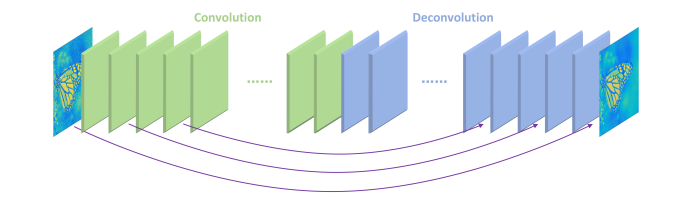
\includegraphics[scale=0.35]{skipconnections_model.png}
		\caption{Skip Connections Model}\label{skips_model}
	\end{figure}
\end{frame}

\begin{frame}
	\frametitle{Skip Connections}
	\begin{columns}
		\begin{column}{0.4\textwidth}
	2 models:
	\begin{equation}
	\begin{split}
		C_{32}^{5,2} - R_{32}^5 - C_{64}^{5,2} - R_{64}^5 - \\ C_{128}^{3,2} - R_{128}^3 - D_{128}^{3,2} - R_{128}^5 -\\ D_{64}^{5,2} - R_{64}^5 - D_{32}^{8,2} - D_{3,p}^{3,1}
	\end{split}
	\label{ResNet_v1}
	\end{equation}

	\begin{equation}
	\begin{split}
		C_{8}^{5,2} - 2R_{8}^5 - C_{16}^{5,2} - 2R_{16}^5 - \\ C_{32}^{3,1} - 2R_{32}^3 - D_{32}^{3,1} - 2R_{32}^5 -\\ D_{16}^{3,1} - 2R_{16}^5 - D_{8}^{8,1} - D_{3,p}^{3,1} 
	\end{split}
	\label{ResNet_v2}
	\end{equation}
	\end{column}
	\begin{column}{0.4\textwidth}
	\begin{figure}[hbtp]
		\centering
		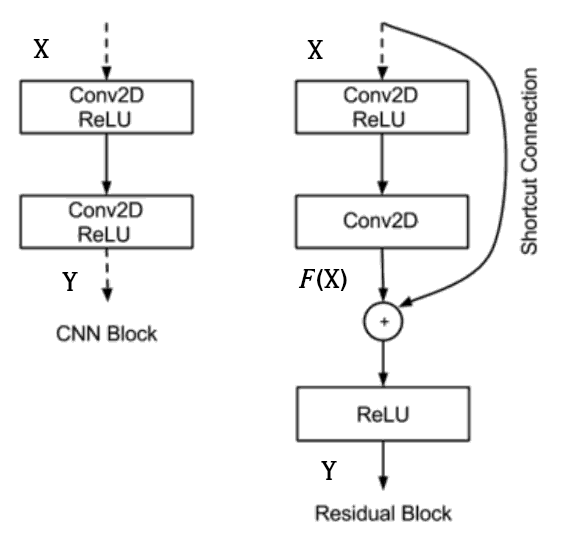
\includegraphics[scale=0.35]{ResidualBlock.png}
		\caption{Residual block}\label{residual_block}
	\end{figure}
	\end{column}
	\end{columns}
\end{frame}

\begin{frame}
	\frametitle{CIFAR10 Results}
	\begin{figure}[hptb]
	\centering
	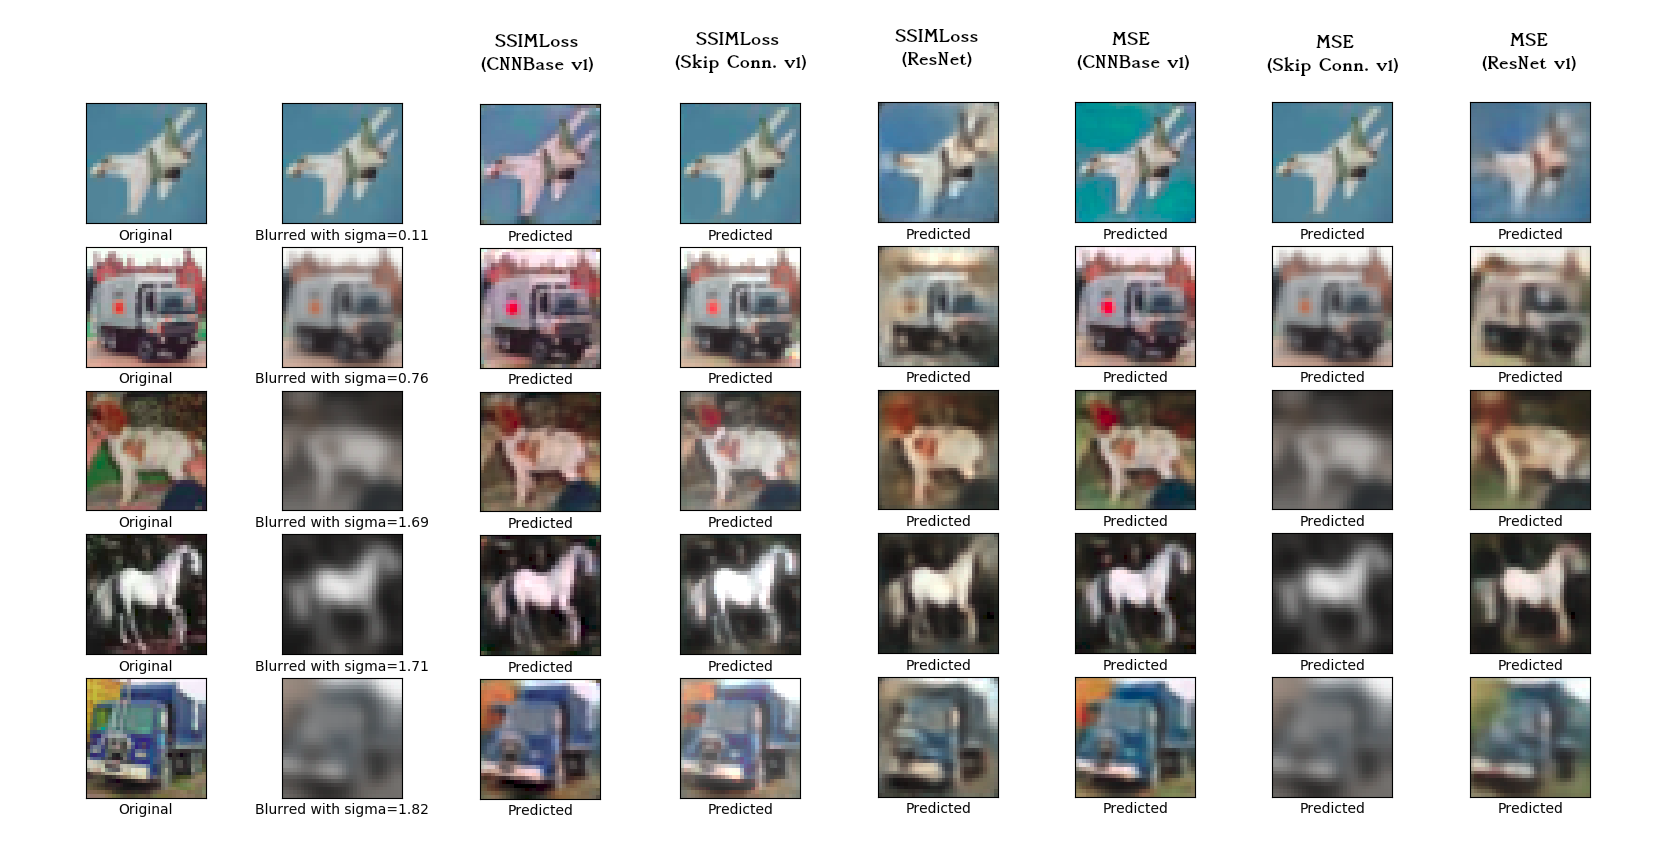
\includegraphics[scale=0.19]{Outputs_comparison.png}
	\caption{Output examples}
	\label{CIFAR10Output}
	\end{figure}
\end{frame}

\begin{frame}
	\frametitle{CIFAR10 Results}
	\begin{figure}[hptb]
	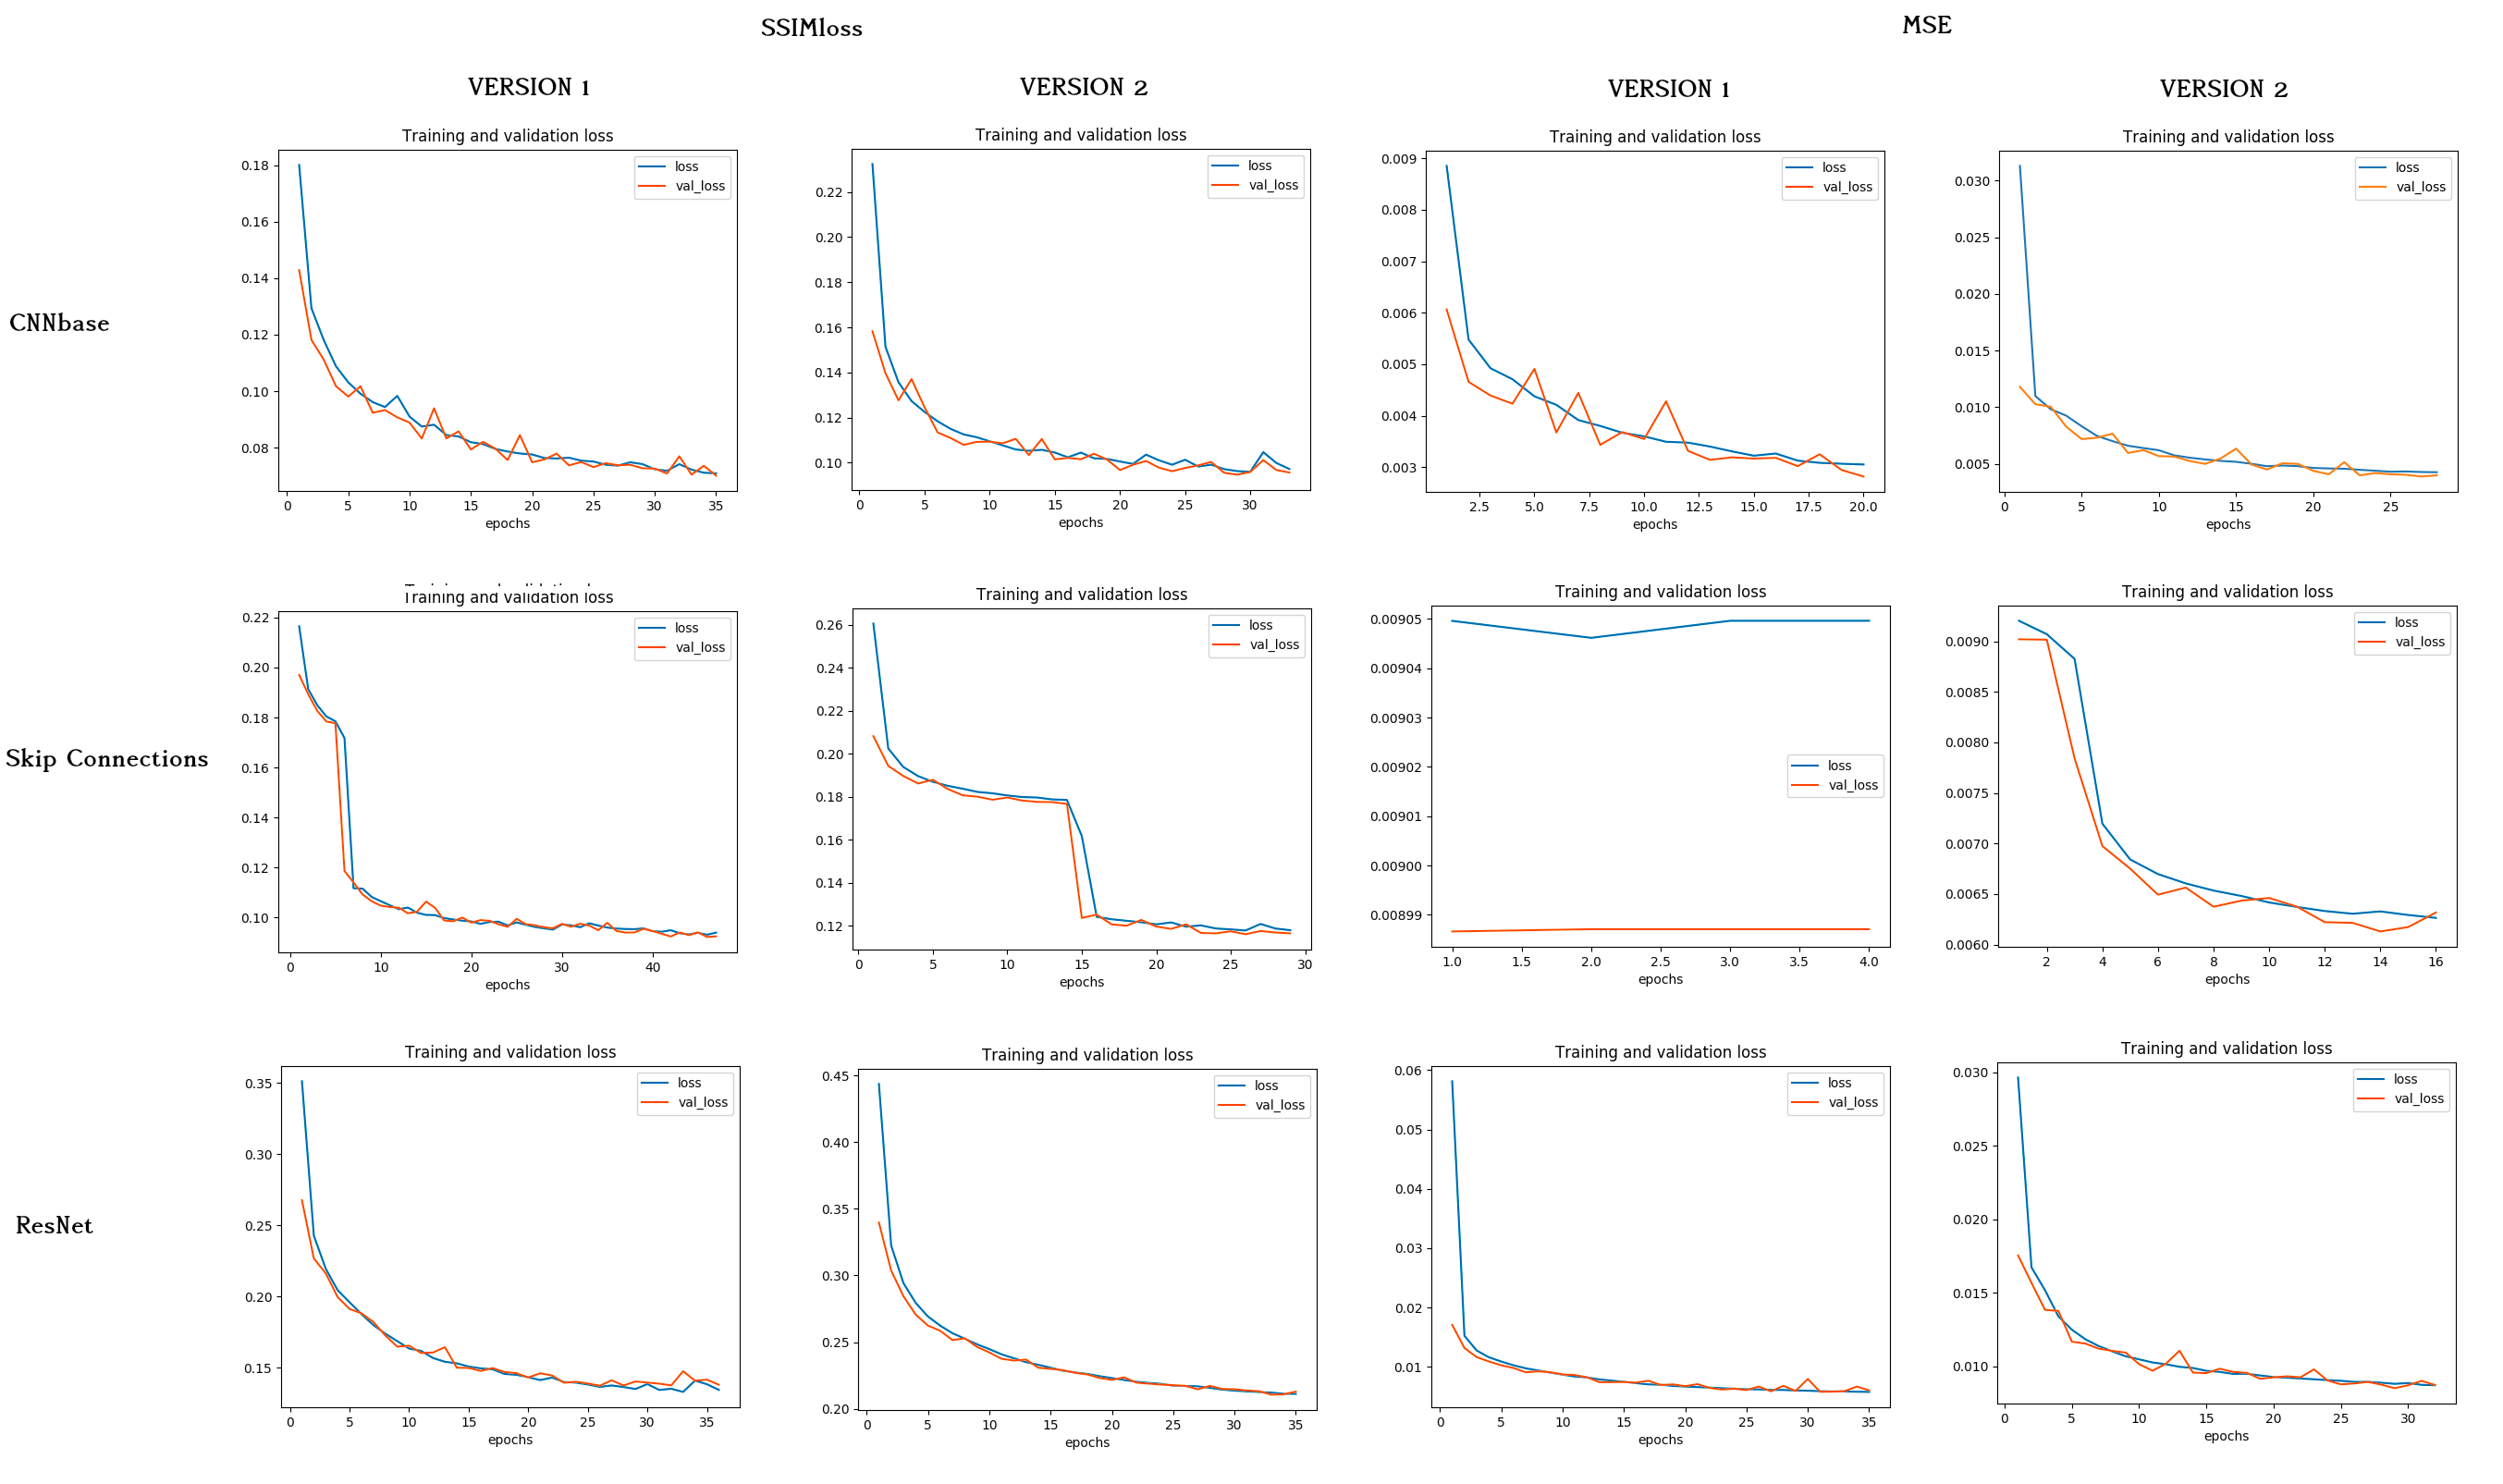
\includegraphics[scale=0.14]{Loss_accuracy_comparison.png}
	\caption{Loss Accuracy Comparison between different networks on CIFAR10}
	\label{CIFAR10Loss}
	\end{figure}
\end{frame}

\begin{frame}
	\frametitle{CIFAR10 Results}
	\begin{figure}[hptb]
	\centering
	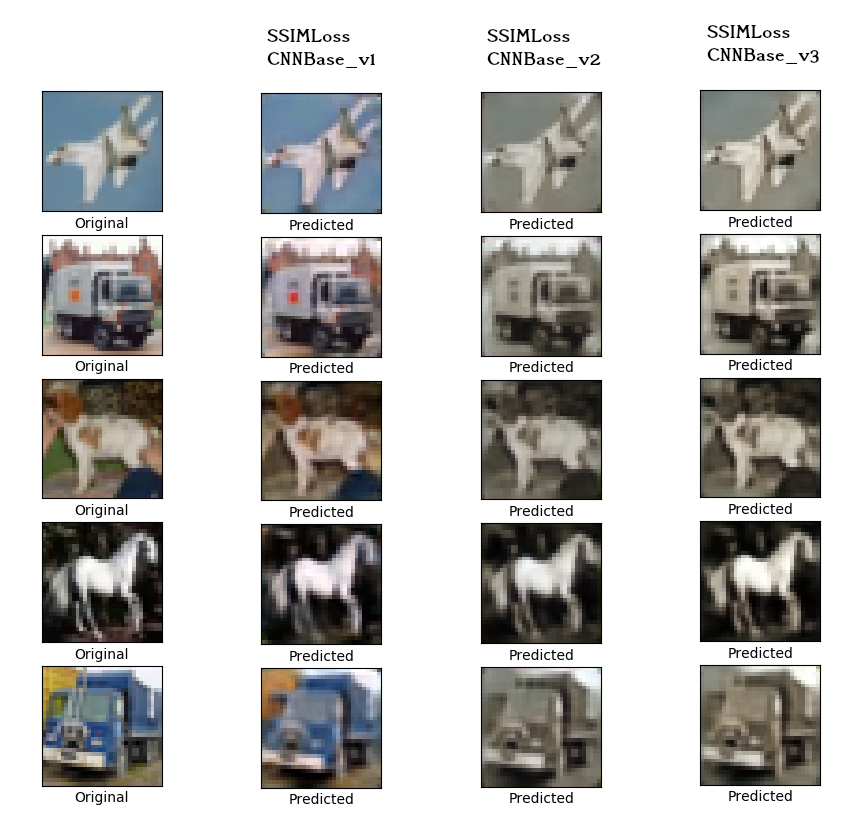
\includegraphics[scale=0.32]{CNNBase_comparison.png}
	\caption{Outputs comparison with different version of CNNBase scheme}
	\label{CNNBase_comparison}
	\end{figure}
\end{frame}


\begin{frame}
	\frametitle{REDs challenges}
	HIGH RESOLUTION IMAGES $\Rightarrow$ HIGH COMPUTATIONAL COST \\
	
	\medskip
	\textbf{Strategies}:
	\begin{itemize}
		\item Virtual Machine on Azure
		\item Local patches 
		\item Training of one version for each architecture with $1-SSIM$ as Loss Function  
	\end{itemize}
\end{frame}

\begin{frame}
	\frametitle{REDs Output I}
	\begin{figure}
		\centering
		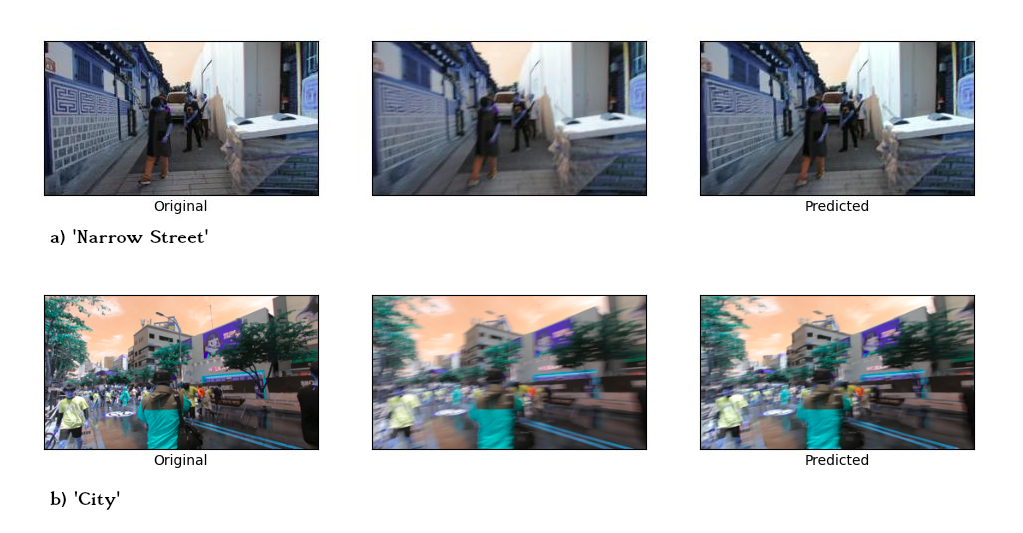
\includegraphics[scale=0.22]{REDs_CNNBase_Outputs.png}
		\tiny{\caption{\textbf{CNN plain network}}}
	\end{figure}		
	
	\begin{figure}
		\centering
		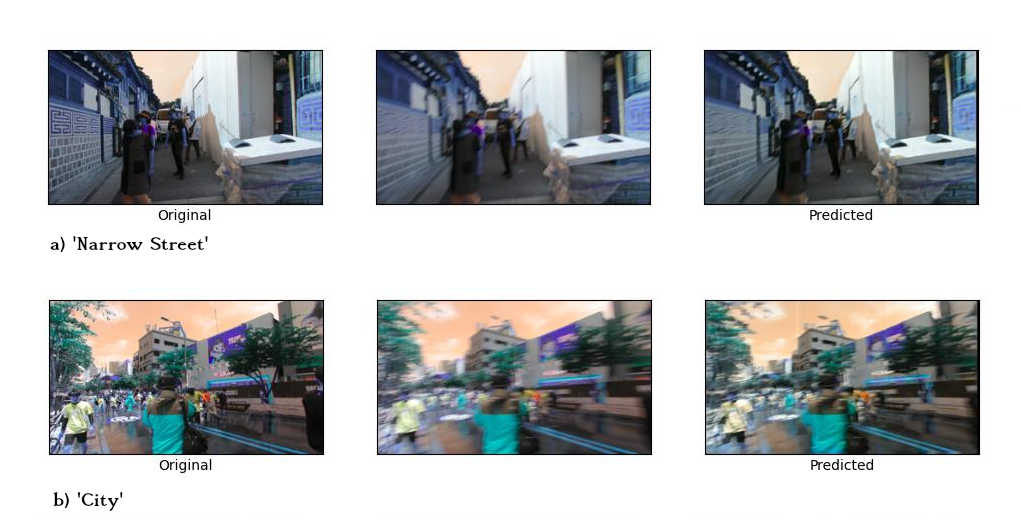
\includegraphics[scale=0.22]{REDs_ResNet_Outputs.png}
		\tiny{\caption{\textbf{ResNet}}}
	\end{figure}		

\end{frame}

	
\begin{frame}
	\frametitle{REDs Output II}
	\begin{figure}
		\centering
		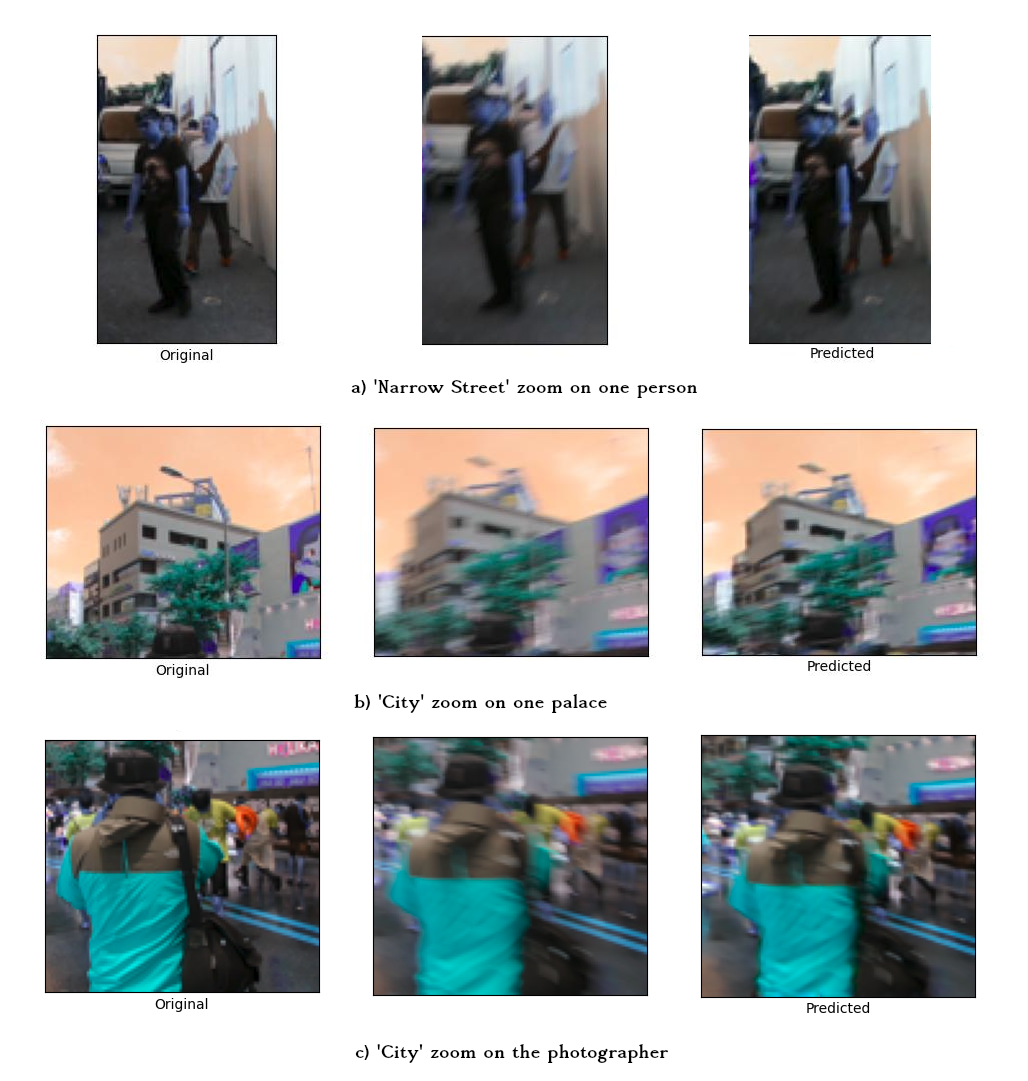
\includegraphics[scale=0.22]{REDs_CNNBase_Outputs_Zoom.png} 
		\tiny{\caption{\textbf{CNN plain network Zoom}}}
	\end{figure}
\end{frame} 


\begin{frame}
	\frametitle{REDs Output III}
	\begin{figure}
		\centering
		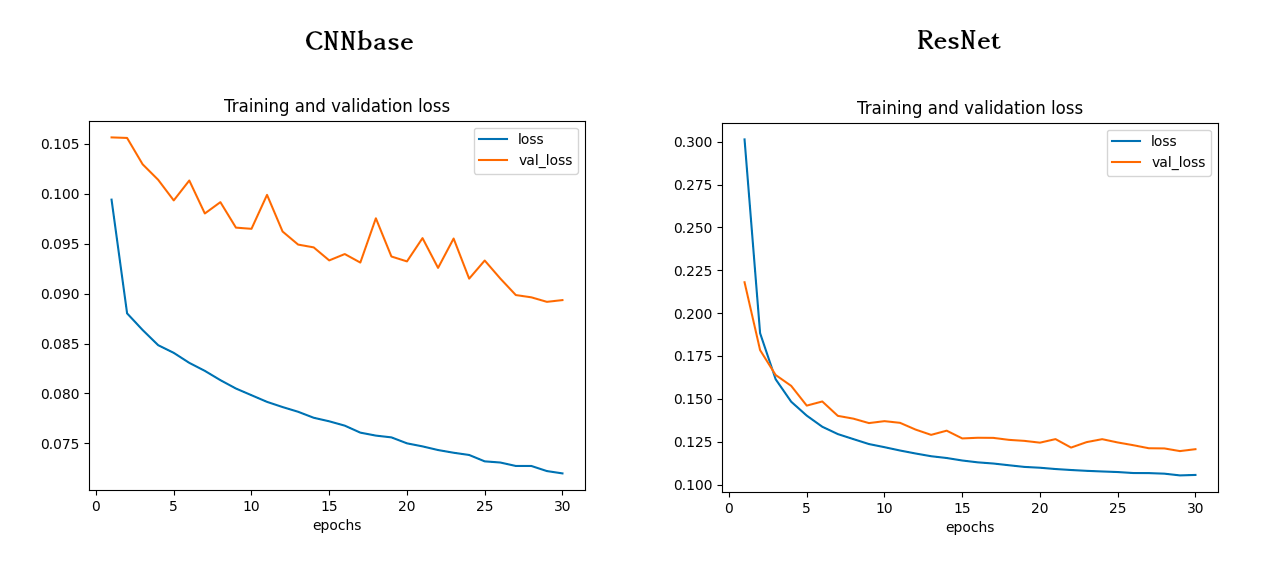
\includegraphics[scale=0.3]{Loss_accuracy_comparison_REDs.png} 
		\tiny{\caption{\textbf{Loss comparison}}}
	\end{figure}
\end{frame}


\begin{frame}
	\frametitle{Other Strategies}
	\begin{columns}
	\begin{column}{0.4\textwidth}
		\begin{figure}
		\centering
		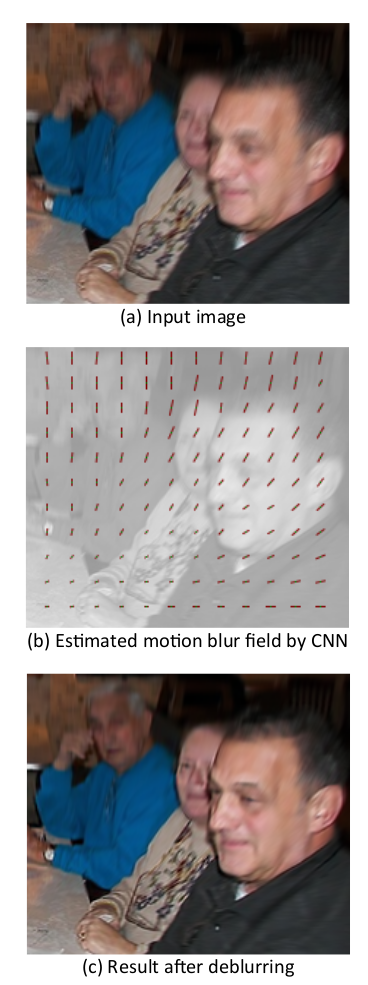
\includegraphics[scale=0.25]{motion_blur_example.png} 
		\tiny{\caption{\textbf{Kernel Motion Estimation}}}
	\end{figure}
	\end{column}
	\begin{column}{0.4\textwidth}
	\begin{figure}
		\centering
		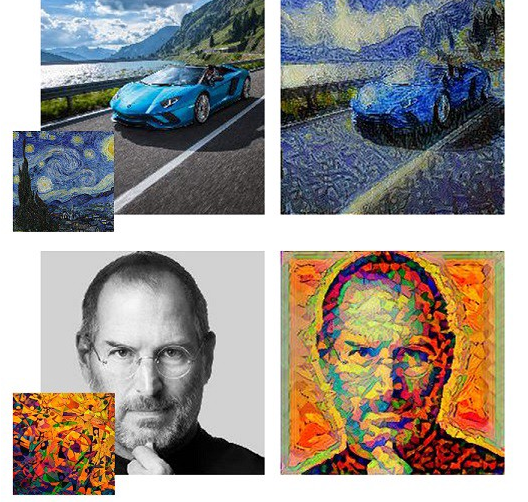
\includegraphics[width=\columnwidth]{style_transfer_example.png} 
		\tiny{\caption{\textbf{Style Transfer}}}
	\end{figure}
	\end{column}
	\end{columns}
\end{frame}


\begin{frame}
	\frametitle{Kernel Motion Approach}
	\begin{figure}[hptb]
	\centering
	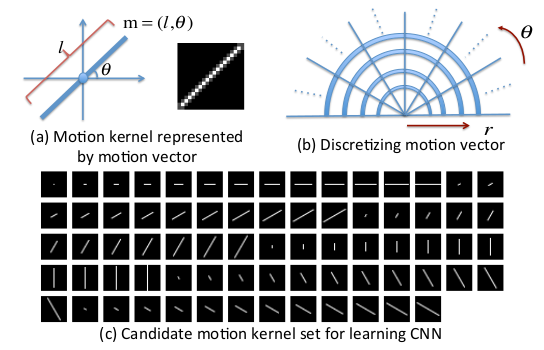
\includegraphics[scale=0.7]{motion_kernel.png} 
	\caption{Representation of motion blur kernel by motion vector
	and generation of motion kernel candidates}
	\label{motion_kernel}
	\end{figure}
\end{frame}

\begin{frame}
	\frametitle{Style Transfer Approach}
	\begin{figure}[hptb]
	\centering
	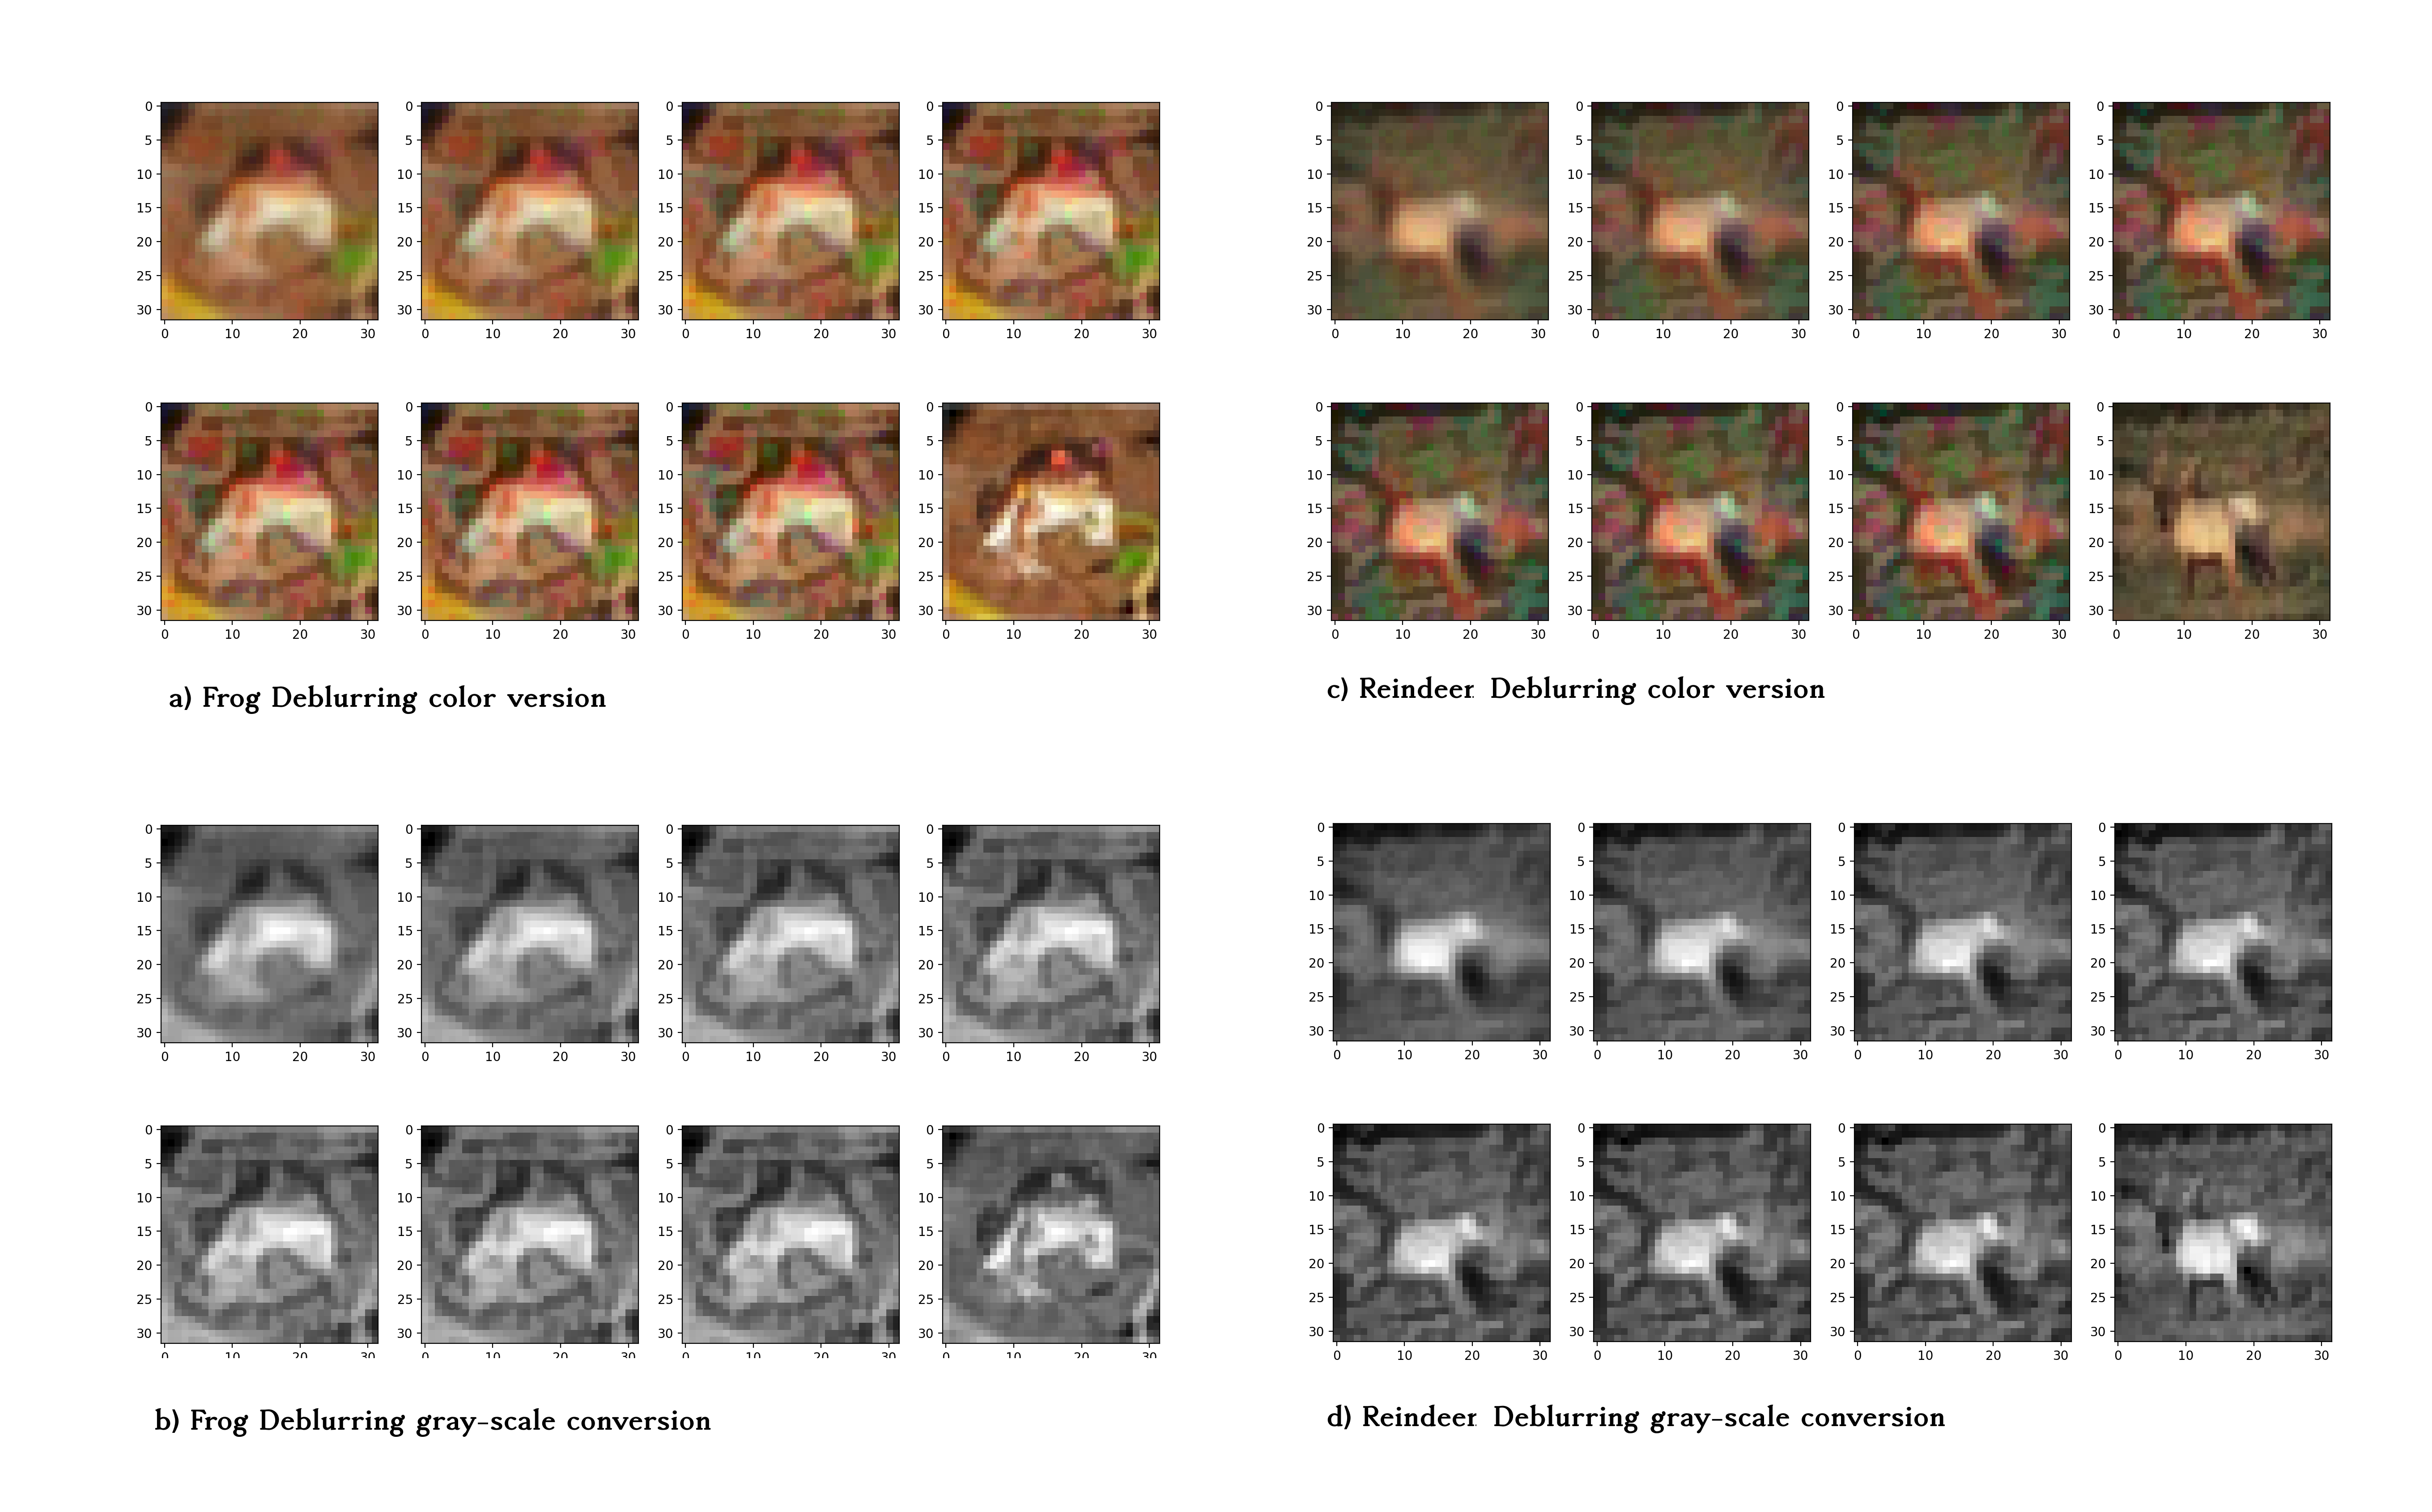
\includegraphics[scale=0.07]{style_outputs.png} 
	\caption{Style Transfer outputs on two images of CIFAR10. The last image in each group is the 	sharp image.}
	\label{style_outputs}
	\end{figure}
\end{frame}


\end{document}